\documentclass[11pt]{beamer}

\usetheme{metropolis}

\usepackage{graphicx}
\usepackage{physics}
\usepackage{adjustbox}
\usepackage{caption}
\usepackage{chemformula}
\usepackage{quoting}
\usepackage{hyperref}
\usepackage[style=chem-angew,backend=bibtex]{biblatex}
\bibliography{references}
%
% Choose how your presentation looks.
%
% For more themes, color themes and font themes, see:
% http://deic.uab.es/~iblanes/beamer_gallery/index_by_theme.html
%
\mode<presentation>
{
  \usetheme{default}      % or try Darmstadt, Madrid, Warsaw, ...
  \usecolortheme{default} % or try albatross, beaver, crane, ...
  \usefonttheme{default}  % or try serif, structurebold, ...
  \setbeamertemplate{navigation symbols}{}
  \setbeamertemplate{caption}[numbered]
  \setbeamerfont{footnote}{size=\tiny}
} 

\usepackage[english]{babel}
\usepackage[utf8]{inputenc}
\graphicspath{{image/}}

\AtBeginSection[]{
\begin{frame}{Outline}
  \tableofcontents[currentsection]
\end{frame}
}

\title{Chapter 1: Matter and Energy}
\institute{Chemistry Department, Cypress College}
\date{August 24, 2022}

\begin{document}

\begin{frame}
  \titlepage
\end{frame}

\begin{frame}{Class Announcements}
  \begin{itemize}
  \item \href{https://www.cypresscollege.edu/academics/divisions-special-programs/librarylrc/library/}
    {chromebook checkout}
  \item Extended due date for the prerequisite scan - provide ID card, transcript
    for algebra class, and the blue worksheet (give 1 EC)
  \item[] \textbf{Canvas}
  \item when2meet office hours survey will be sent out after class
  \item Lecture slides will be posted after class
  \item First quiz will be posted Thurs at 11am and you have until Mon, Aug 29th
    at 11:59pm
  \item First homework assignment posted Fri, Aug 26th at 3pm
  \end{itemize}
\end{frame}

\section{Review: Scientific Notation and Unit Conversion}

\begin{frame}{Recap: Building the Mathematical Toolbox}
  \begin{itemize}
  \item Scientific notation simplifies large numbers to
    a manageable one
  \item Significant figures imply accuracy
    \begin{itemize}
    \item Leading, sandwiched, and trailing zeroes
    \item Addition and subtraction round to the fewest digits
      after the decimal
    \item Multiplication and division round to the least significant
      digit
    \end{itemize}
  \item Unit conversion - \textit{familiarize} the metric system
    e.g. Gm, Mm, km, m, dm, cm, ...
  \end{itemize}
\end{frame}

\begin{frame}{Prefixes of Metric System}
  \centering
  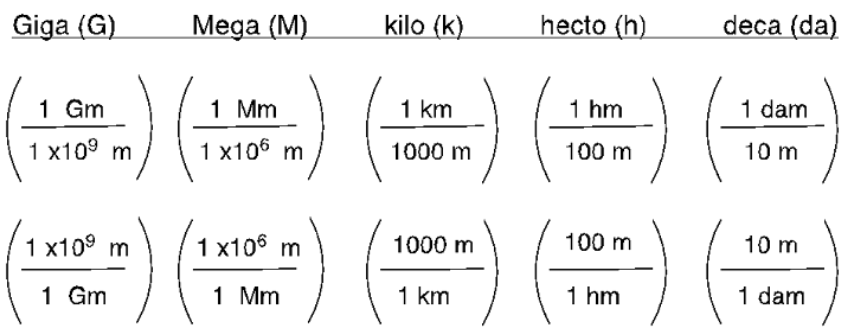
\includegraphics[scale=0.3]{metric_1}
  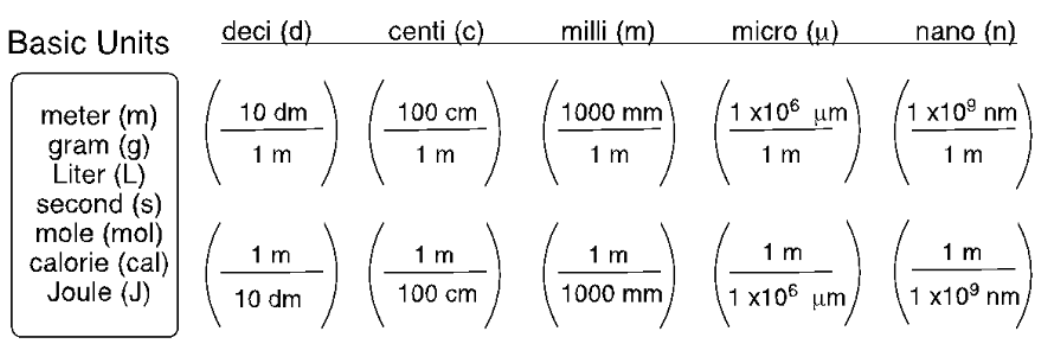
\includegraphics[scale=0.3]{metric_2}
\end{frame}

\begin{frame}{Quick Practice: Significant Figures}
  \centering
  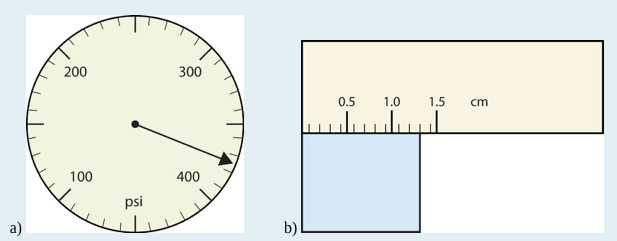
\includegraphics[scale=0.45]{instrument_sig}
\end{frame}

\begin{frame}{Strategy for Dimensional Analysis}
  \begin{enumerate}
  \item Identify the information given and the
    information needed to answer.
  \item Find the relationship(s) between the known
    information and unknown answer, and plan a series
    of steps, including conversion factors, for getting from
    one to the other.
  \item Solve the problem by canceling units.
  \item Check the answer to make sure it makes sense,
    both in magnitude and units.
  \end{enumerate}
\end{frame}

\begin{frame}{Whiteboard: Sig Figs and Dimensional Analysis}
\end{frame}

\section{Matter and Its Classification}

\begin{frame}{Chemistry is Everywhere!}
  \centering
  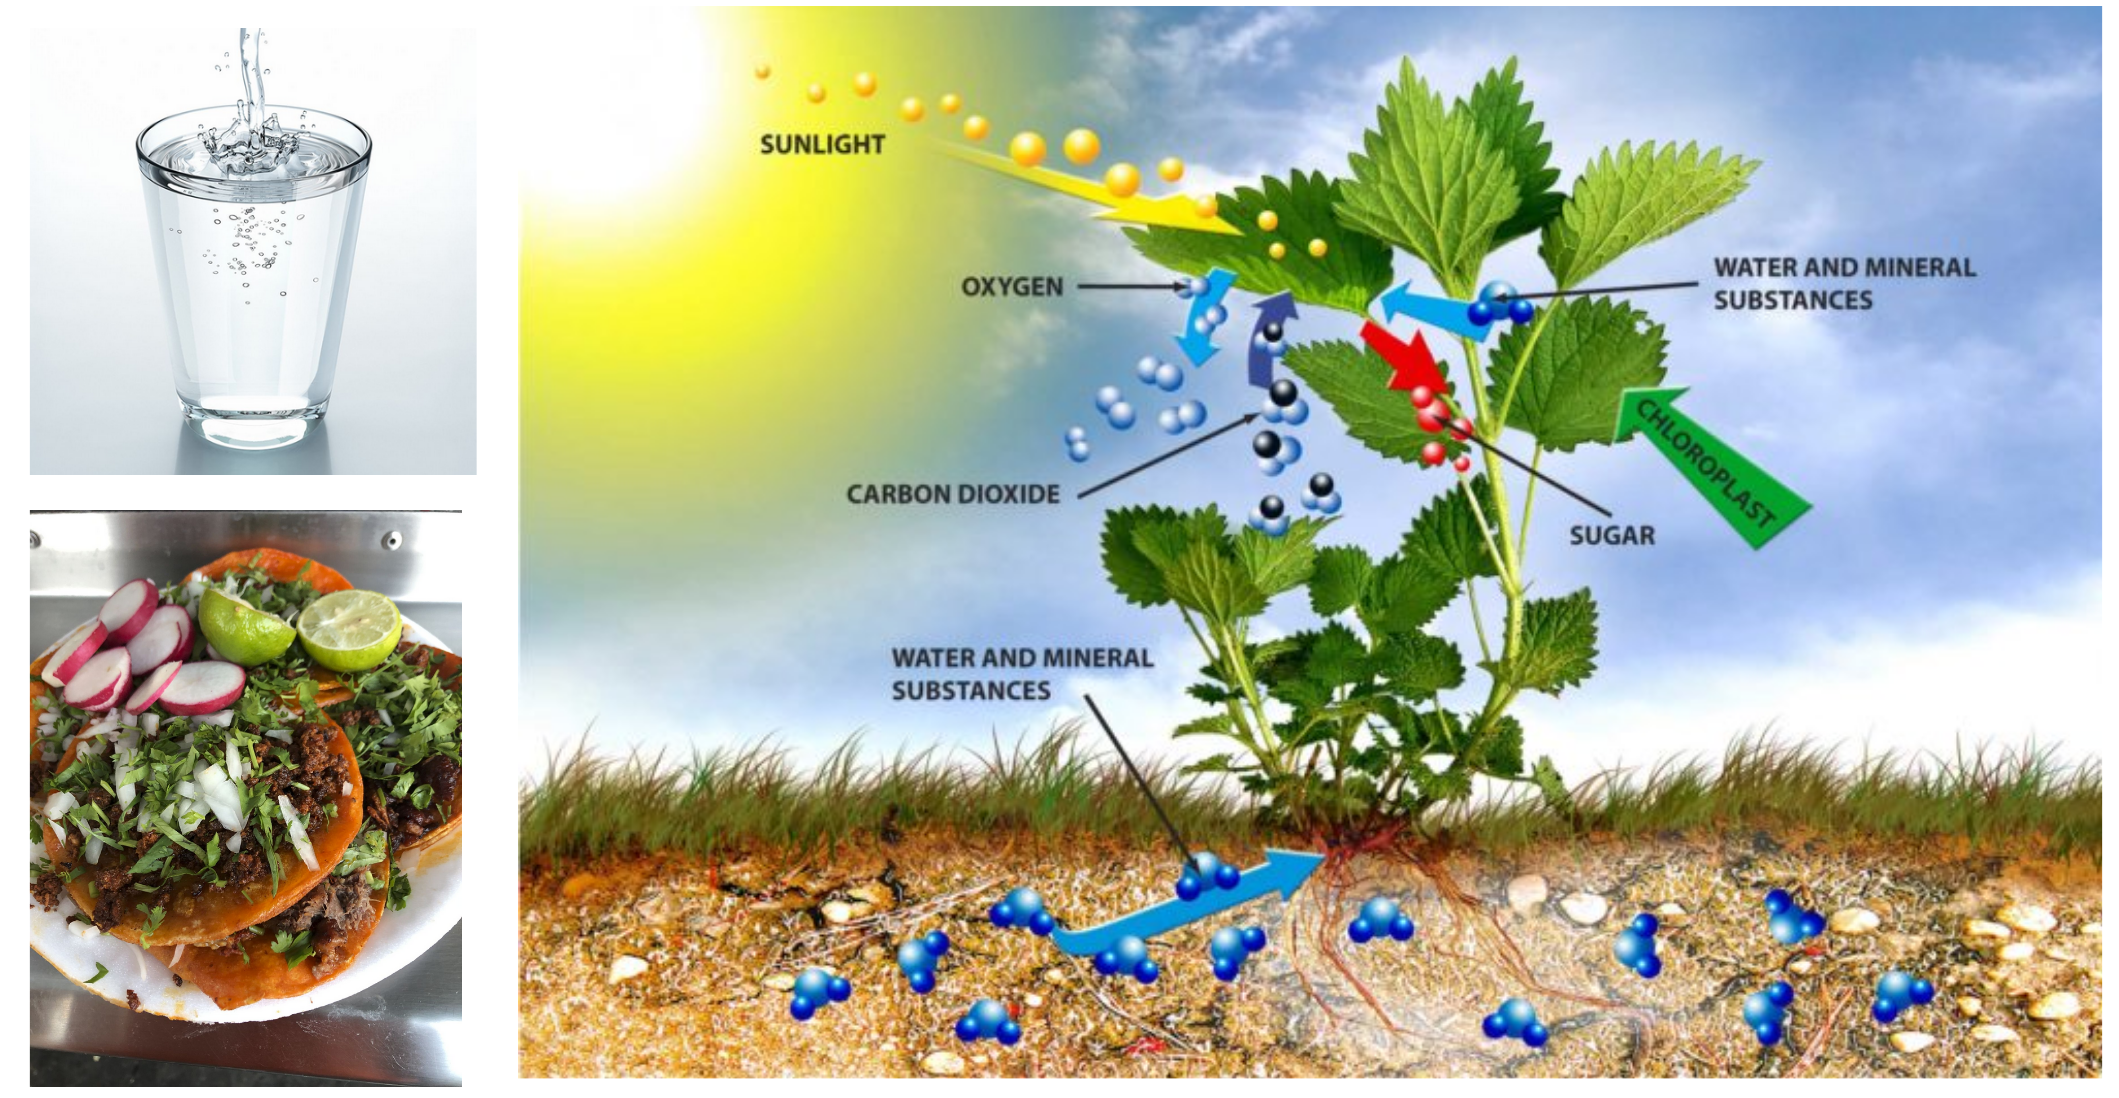
\includegraphics[width=1\linewidth]{food_pic}
\end{frame}

\begin{frame}{Conservation of Mass}
  Any system closed to all transfers of matter and energy, the mass
  of the system must remain constant over time
\end{frame}

\begin{frame}{Classification: Composition of Matter}
  \textbf{Pure substance} - cannot be separated into components

  \textbf{Mixture} - consists at least 2 pure substances mixed
  together
\end{frame}

\begin{frame}{Classification: Composition of Matter}
  \textbf{Pure substance} - cannot be separated into components
  
  Checkout the preiodic table (\href{https://ptable.com}{ptable})
  
  \centering
  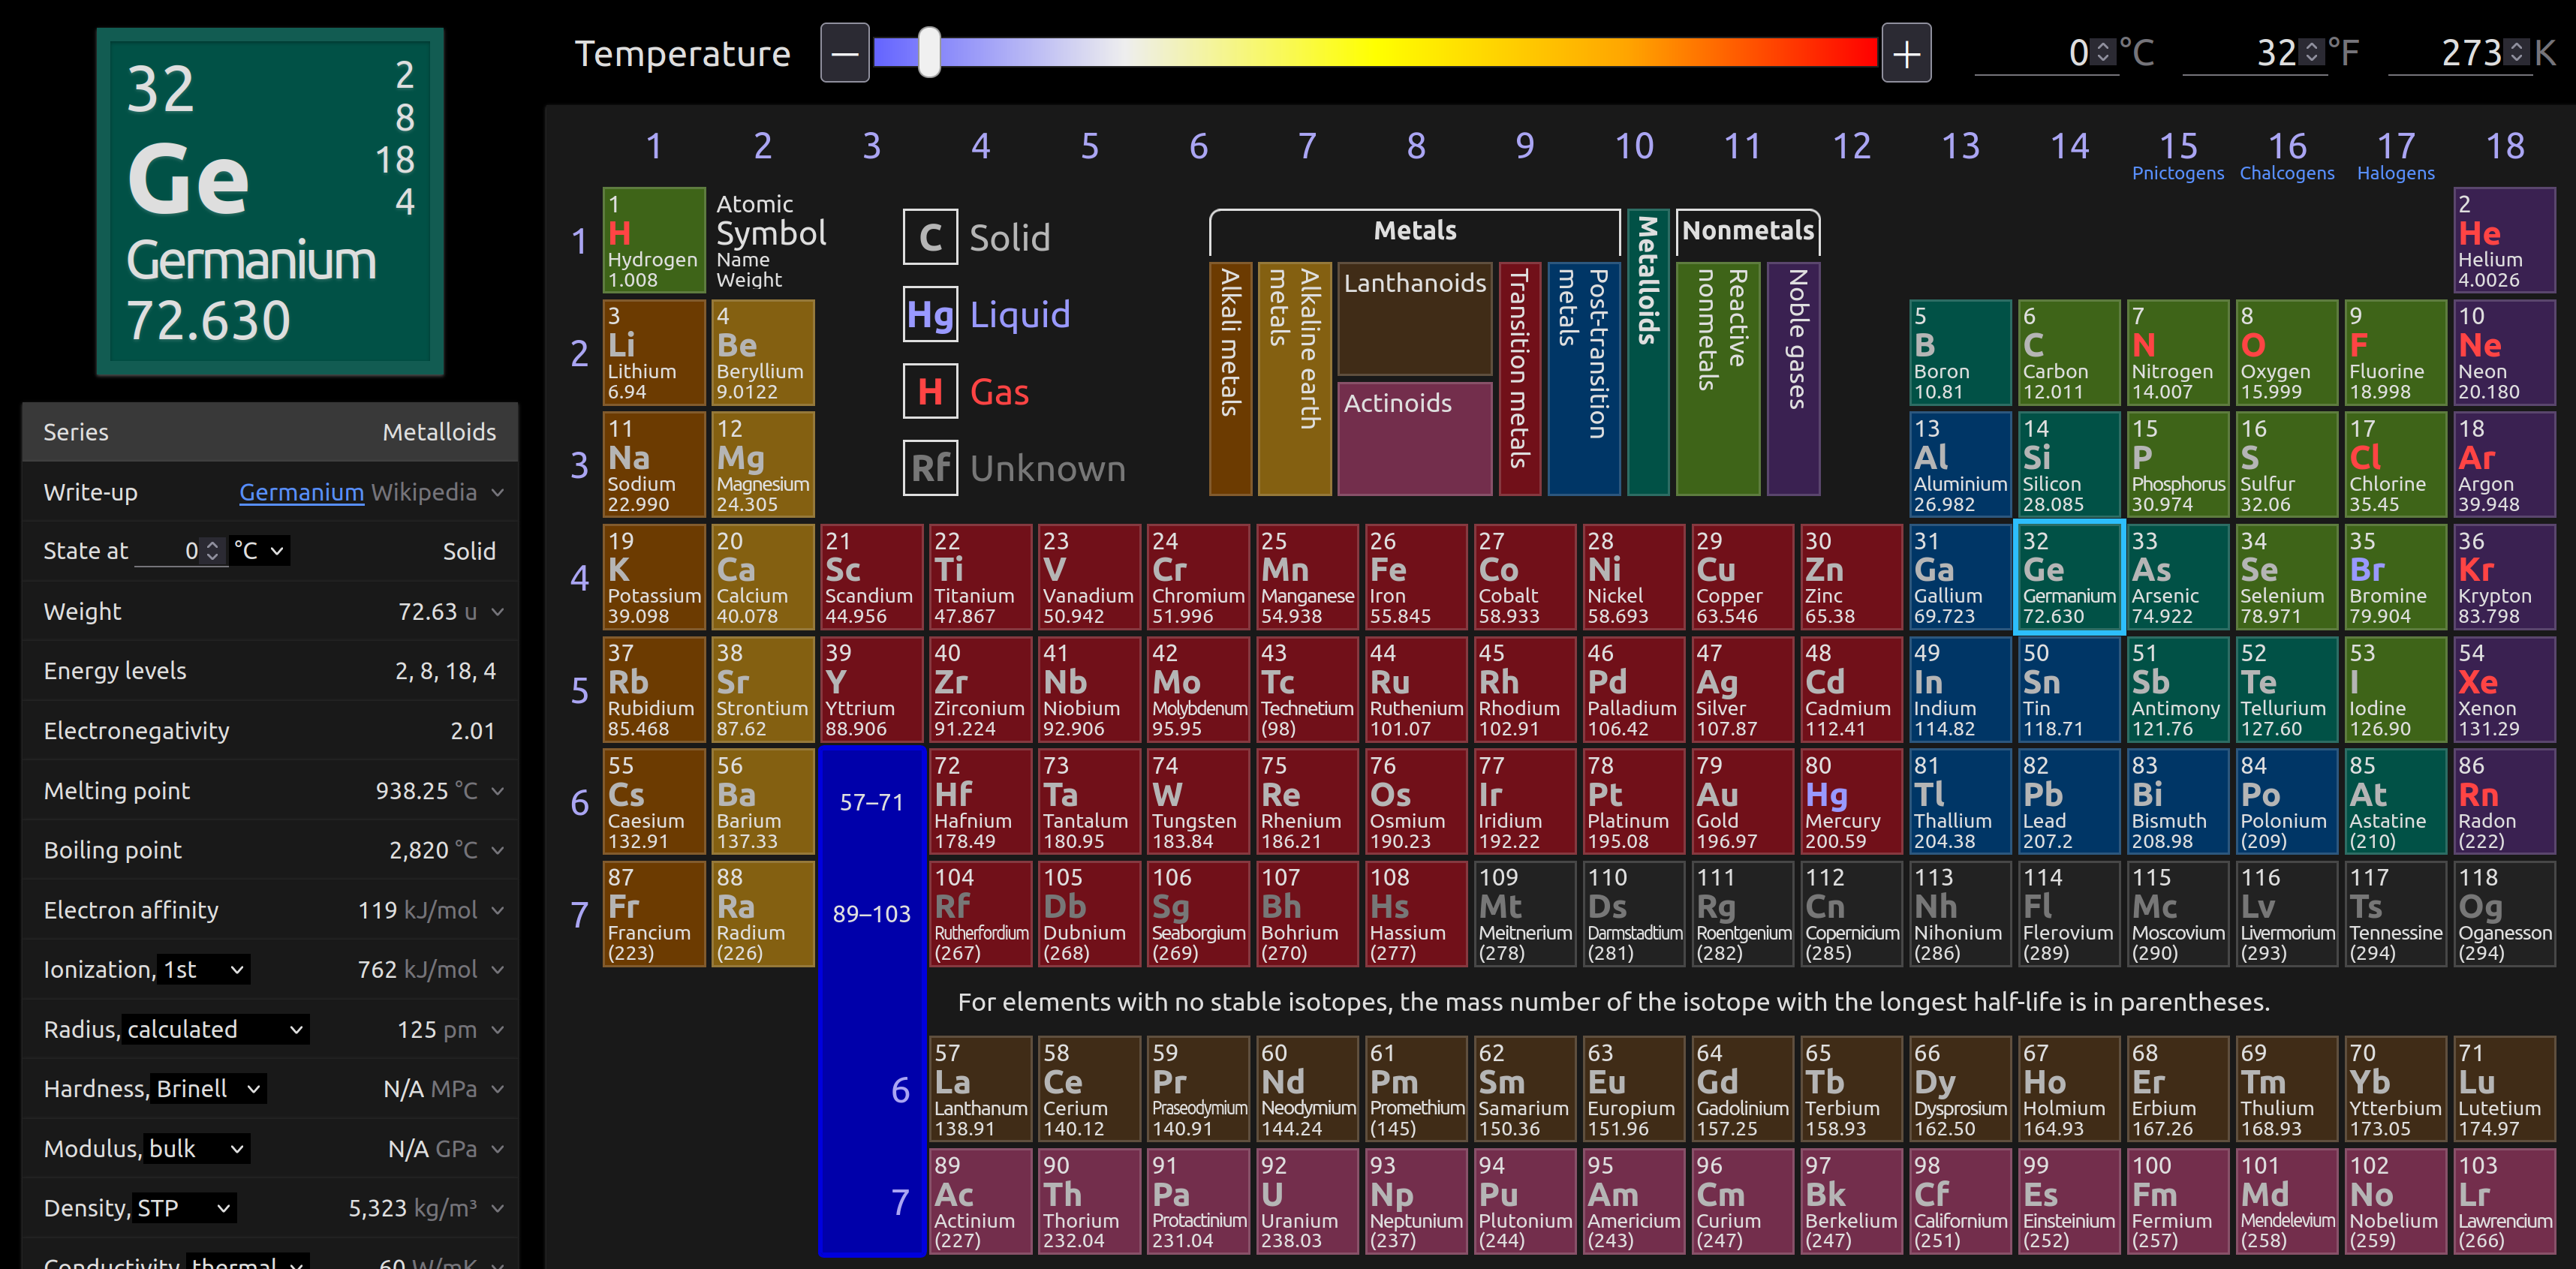
\includegraphics[width=\linewidth]{ptable}
\end{frame}

\begin{frame}{Examples of Pure Substances}
  \centering
  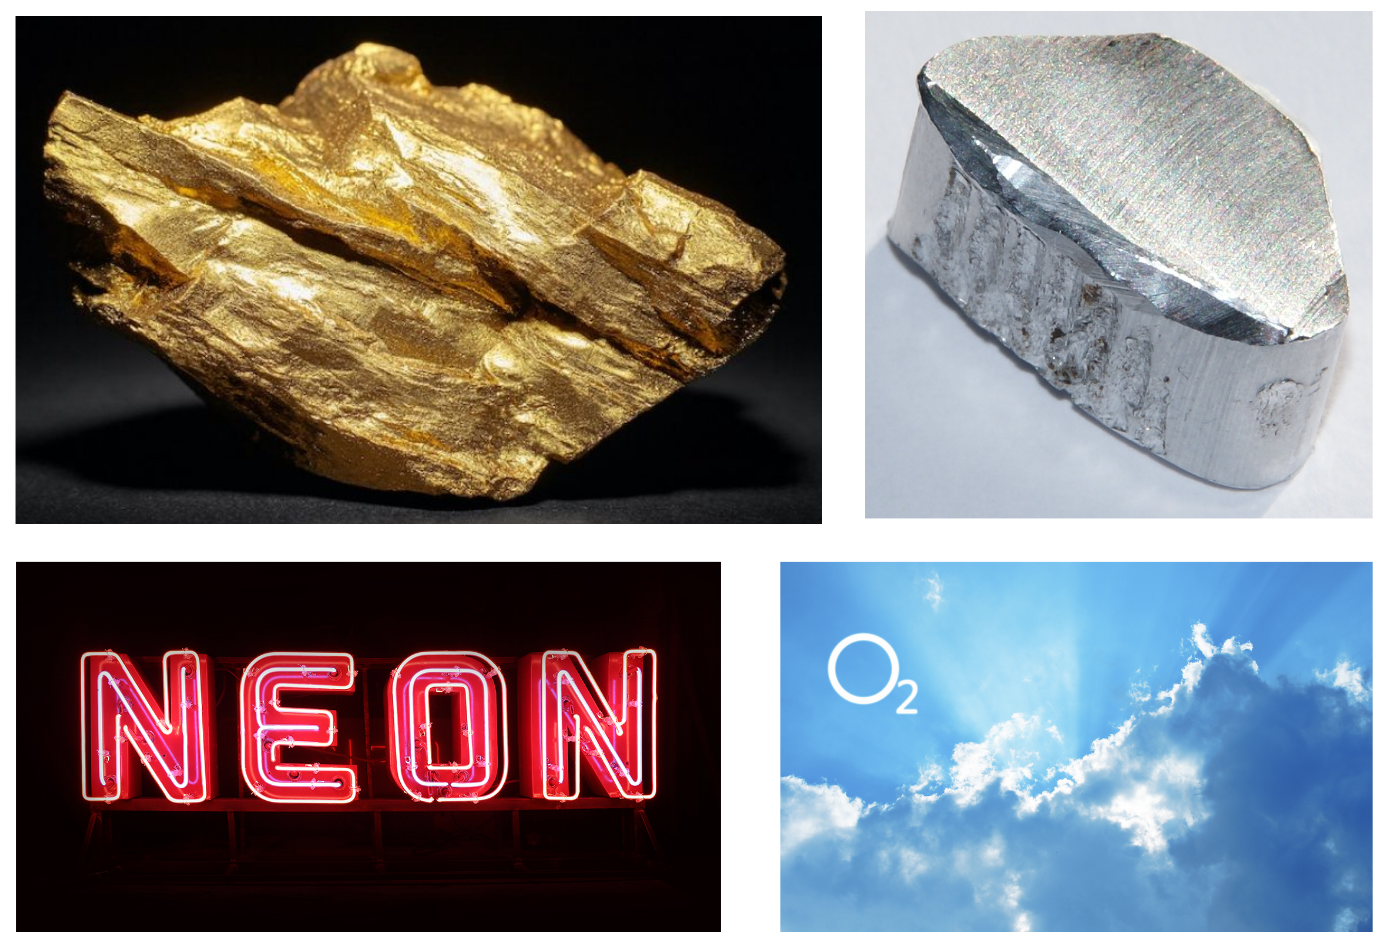
\includegraphics[width=\linewidth]{pure}
\end{frame}

\begin{frame}{Is water a pure substance?}
  \centering
  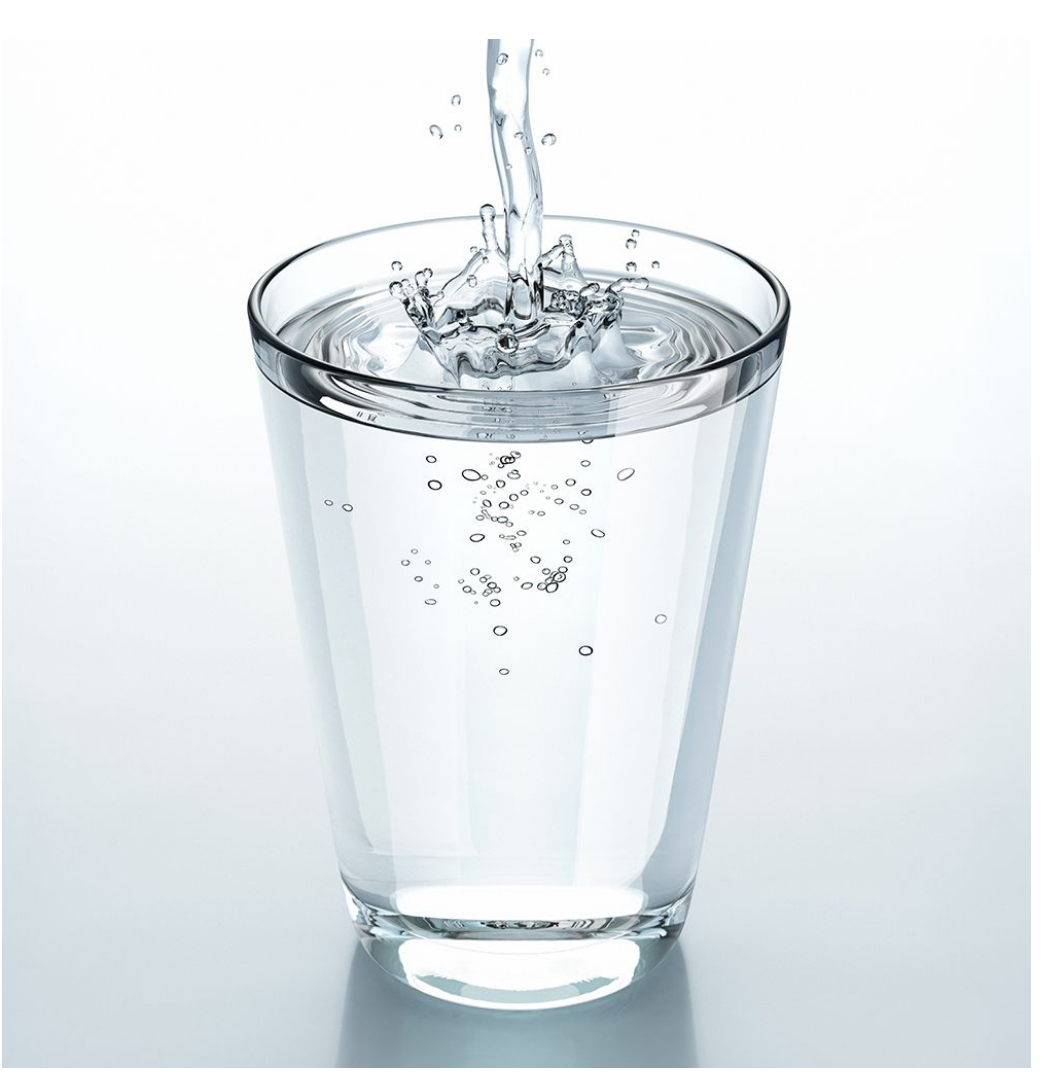
\includegraphics[scale=0.2]{water}
\end{frame}

\begin{frame}{Types of Mixtures}
  \centering
  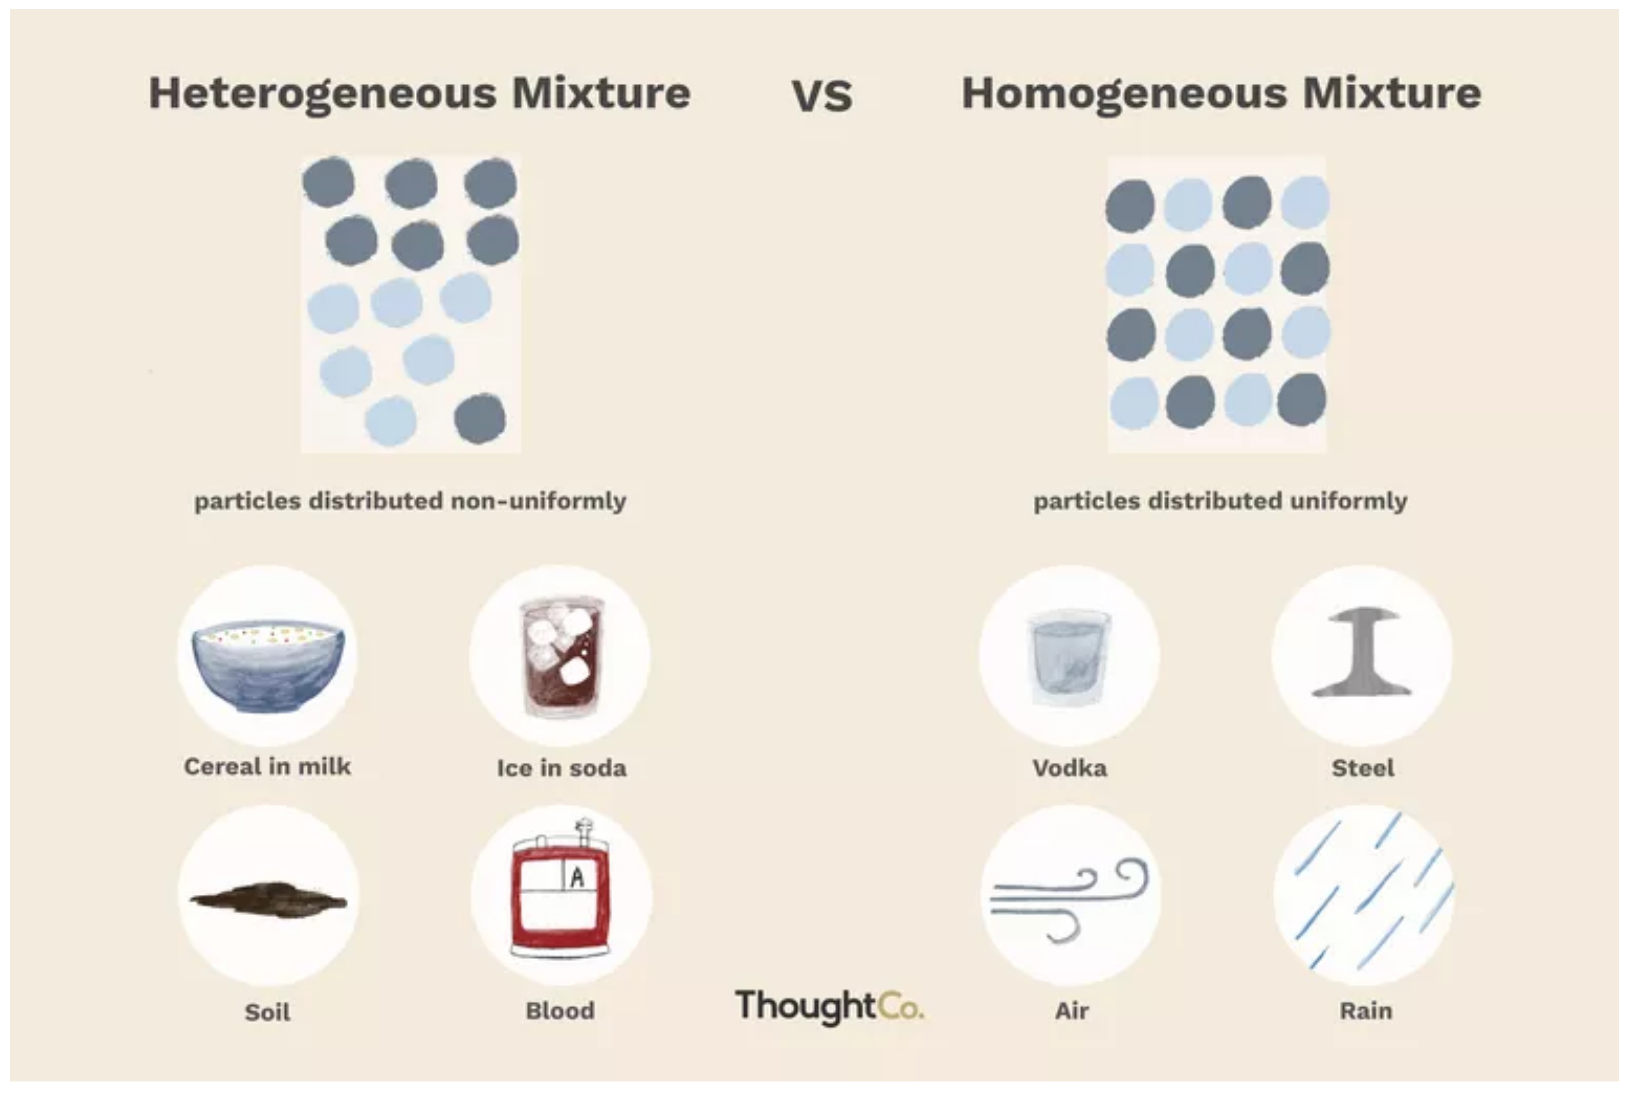
\includegraphics[width=\linewidth]{mixtures}
\end{frame}

\begin{frame}{Mixture Flowchart}
  \centering
  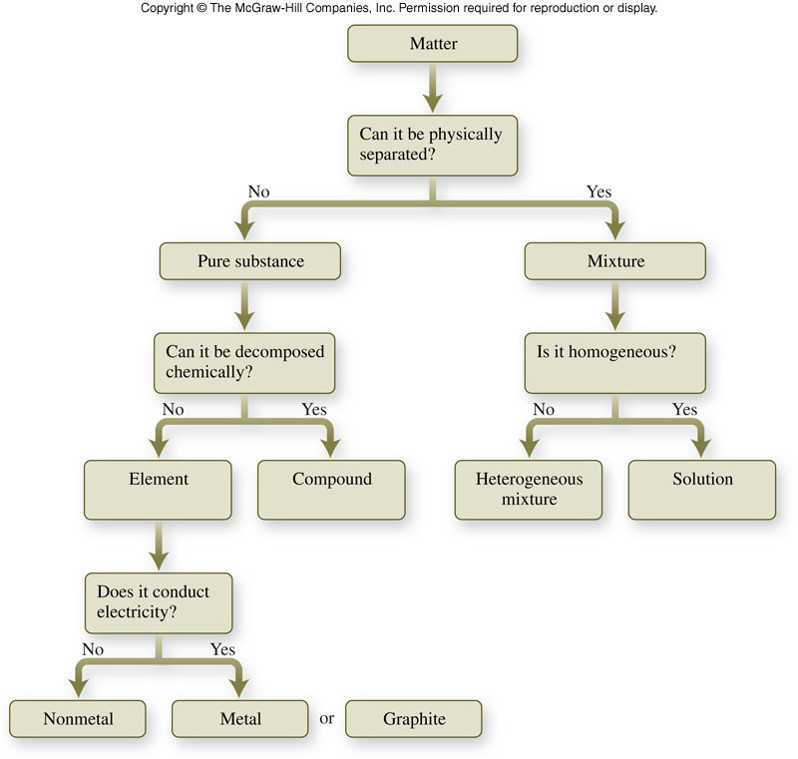
\includegraphics[width=0.8\linewidth]{mix_flowchart}
\end{frame}

\begin{frame}{States of Matter: Water}
  \centering
  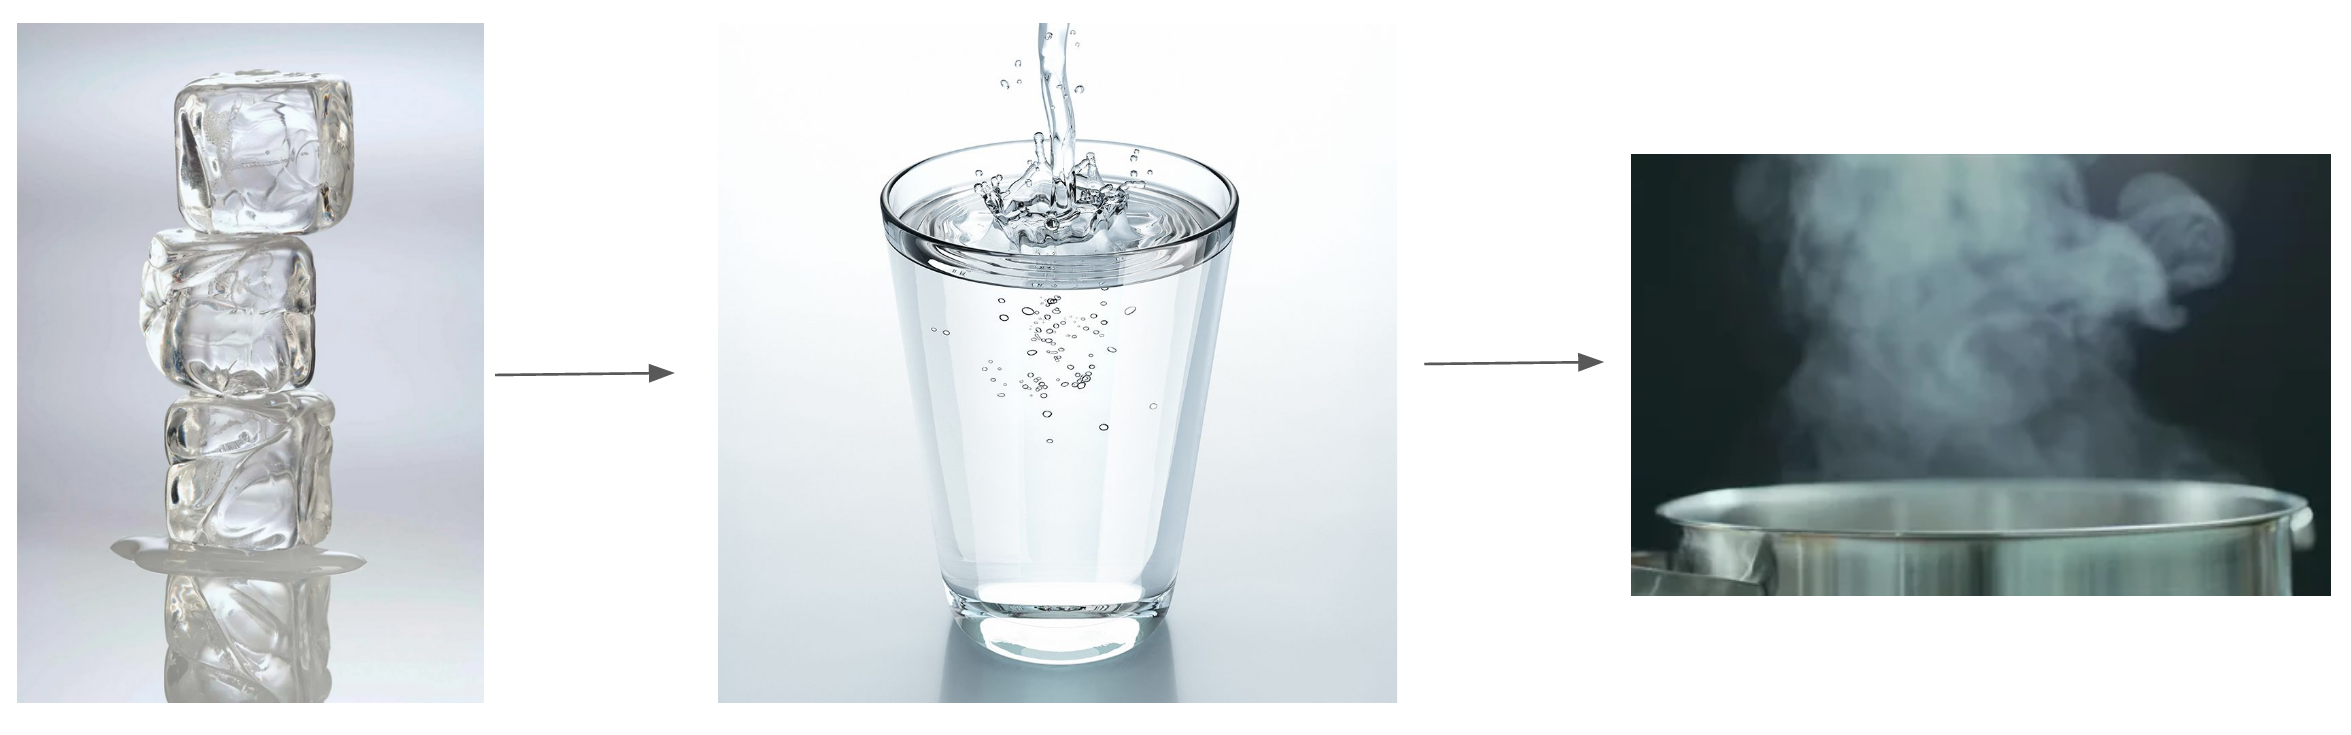
\includegraphics[width=\linewidth]{water_states}
  \vspace{-0.2in}
  \begin{itemize}
  \item Solid has the smallest volume whereas gas occupies
    the largest space
  \item Water molecules have the most energy in which state?
  \item Notation for states - H$_2$O(s), H$_2$O(l), H$_2$O(g)
  \item \textbf{Aqueous state} - substance dissolved in water
    e.g. NaCl(aq)
  \end{itemize}
\end{frame}

\section{Chemical and Physical Changes}

\begin{frame}{Physical Properties}
  A characteristic that can be observed or measured without
  changing the composition of a substance
  
  \centering
  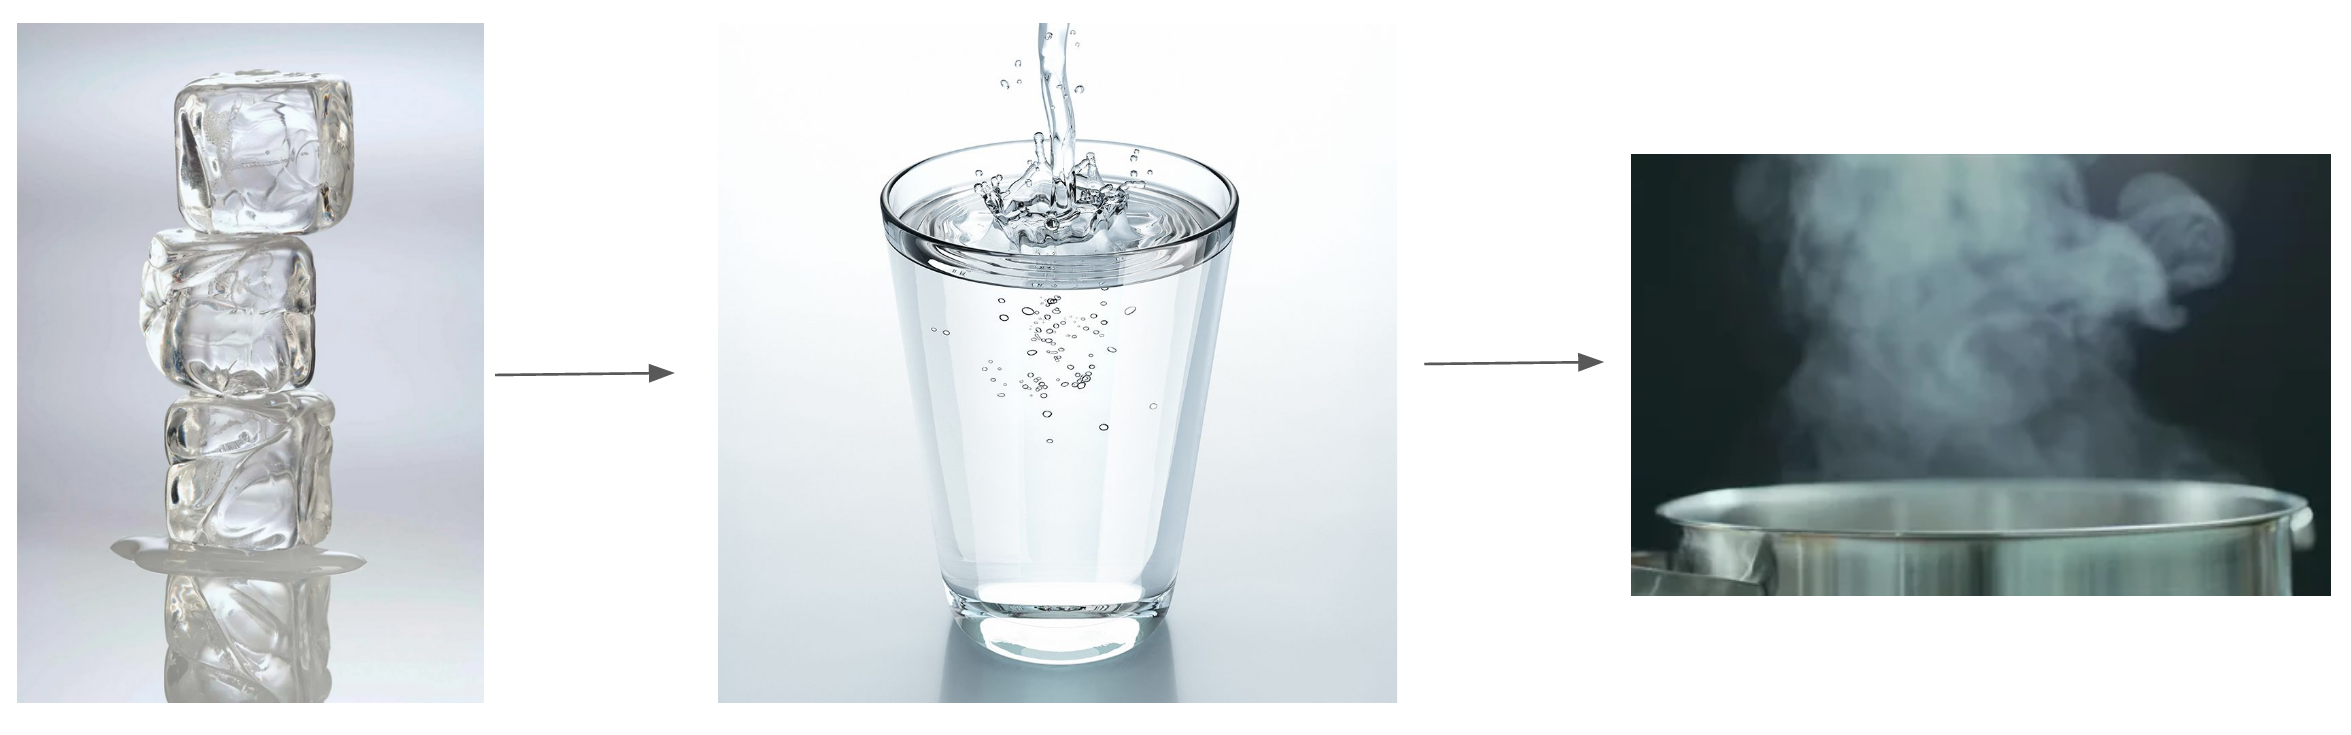
\includegraphics[width=\linewidth]{water_states}
\end{frame}

\begin{frame}{Quantifying Physical Properties}
  \begin{itemize}
  \item Mass - quantifies matter; measuring in grams
  \item Volumne - amount of space occupied; measuring in L
  \item Density - ratio of mass and volume
  \end{itemize}
  \centering
  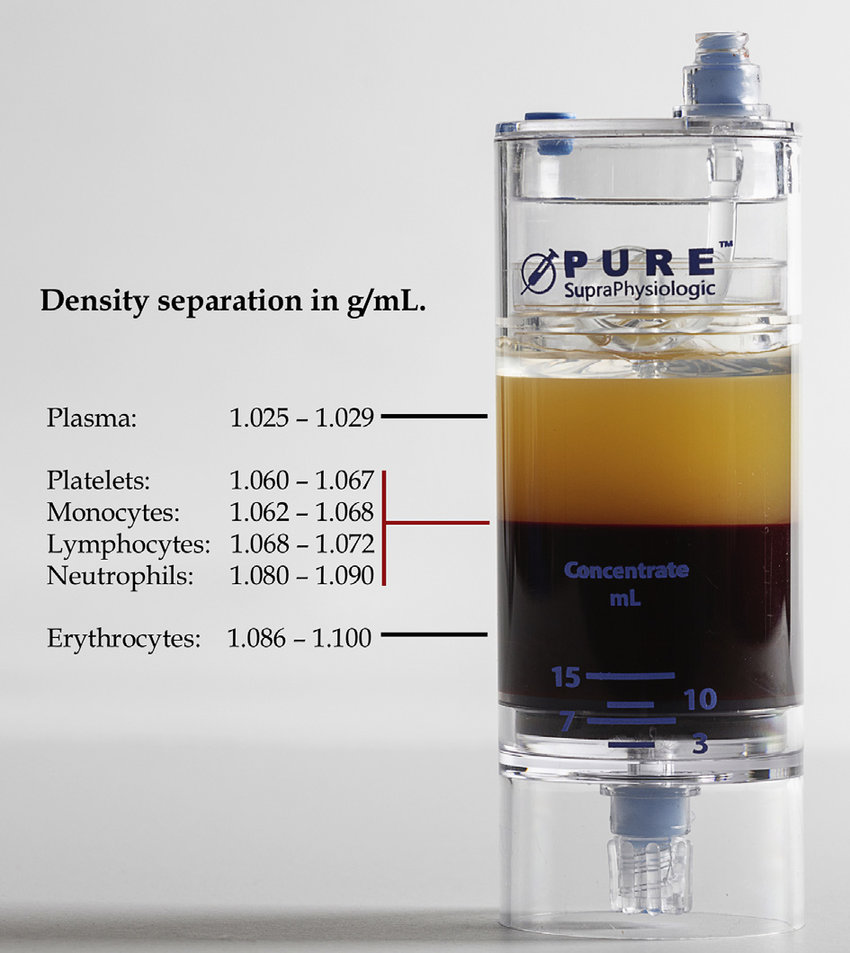
\includegraphics[scale=0.14]{dens_liquids}
  \begin{itemize}
  \item Temperature - quantifies the intensity of heat in a substance
    or object
  \end{itemize}
\end{frame}

\begin{frame}{Chemical Properties}
  A characteristic of a particular subtance that can be observed
  in a chemical reaction e.g. combustion

  \centering
  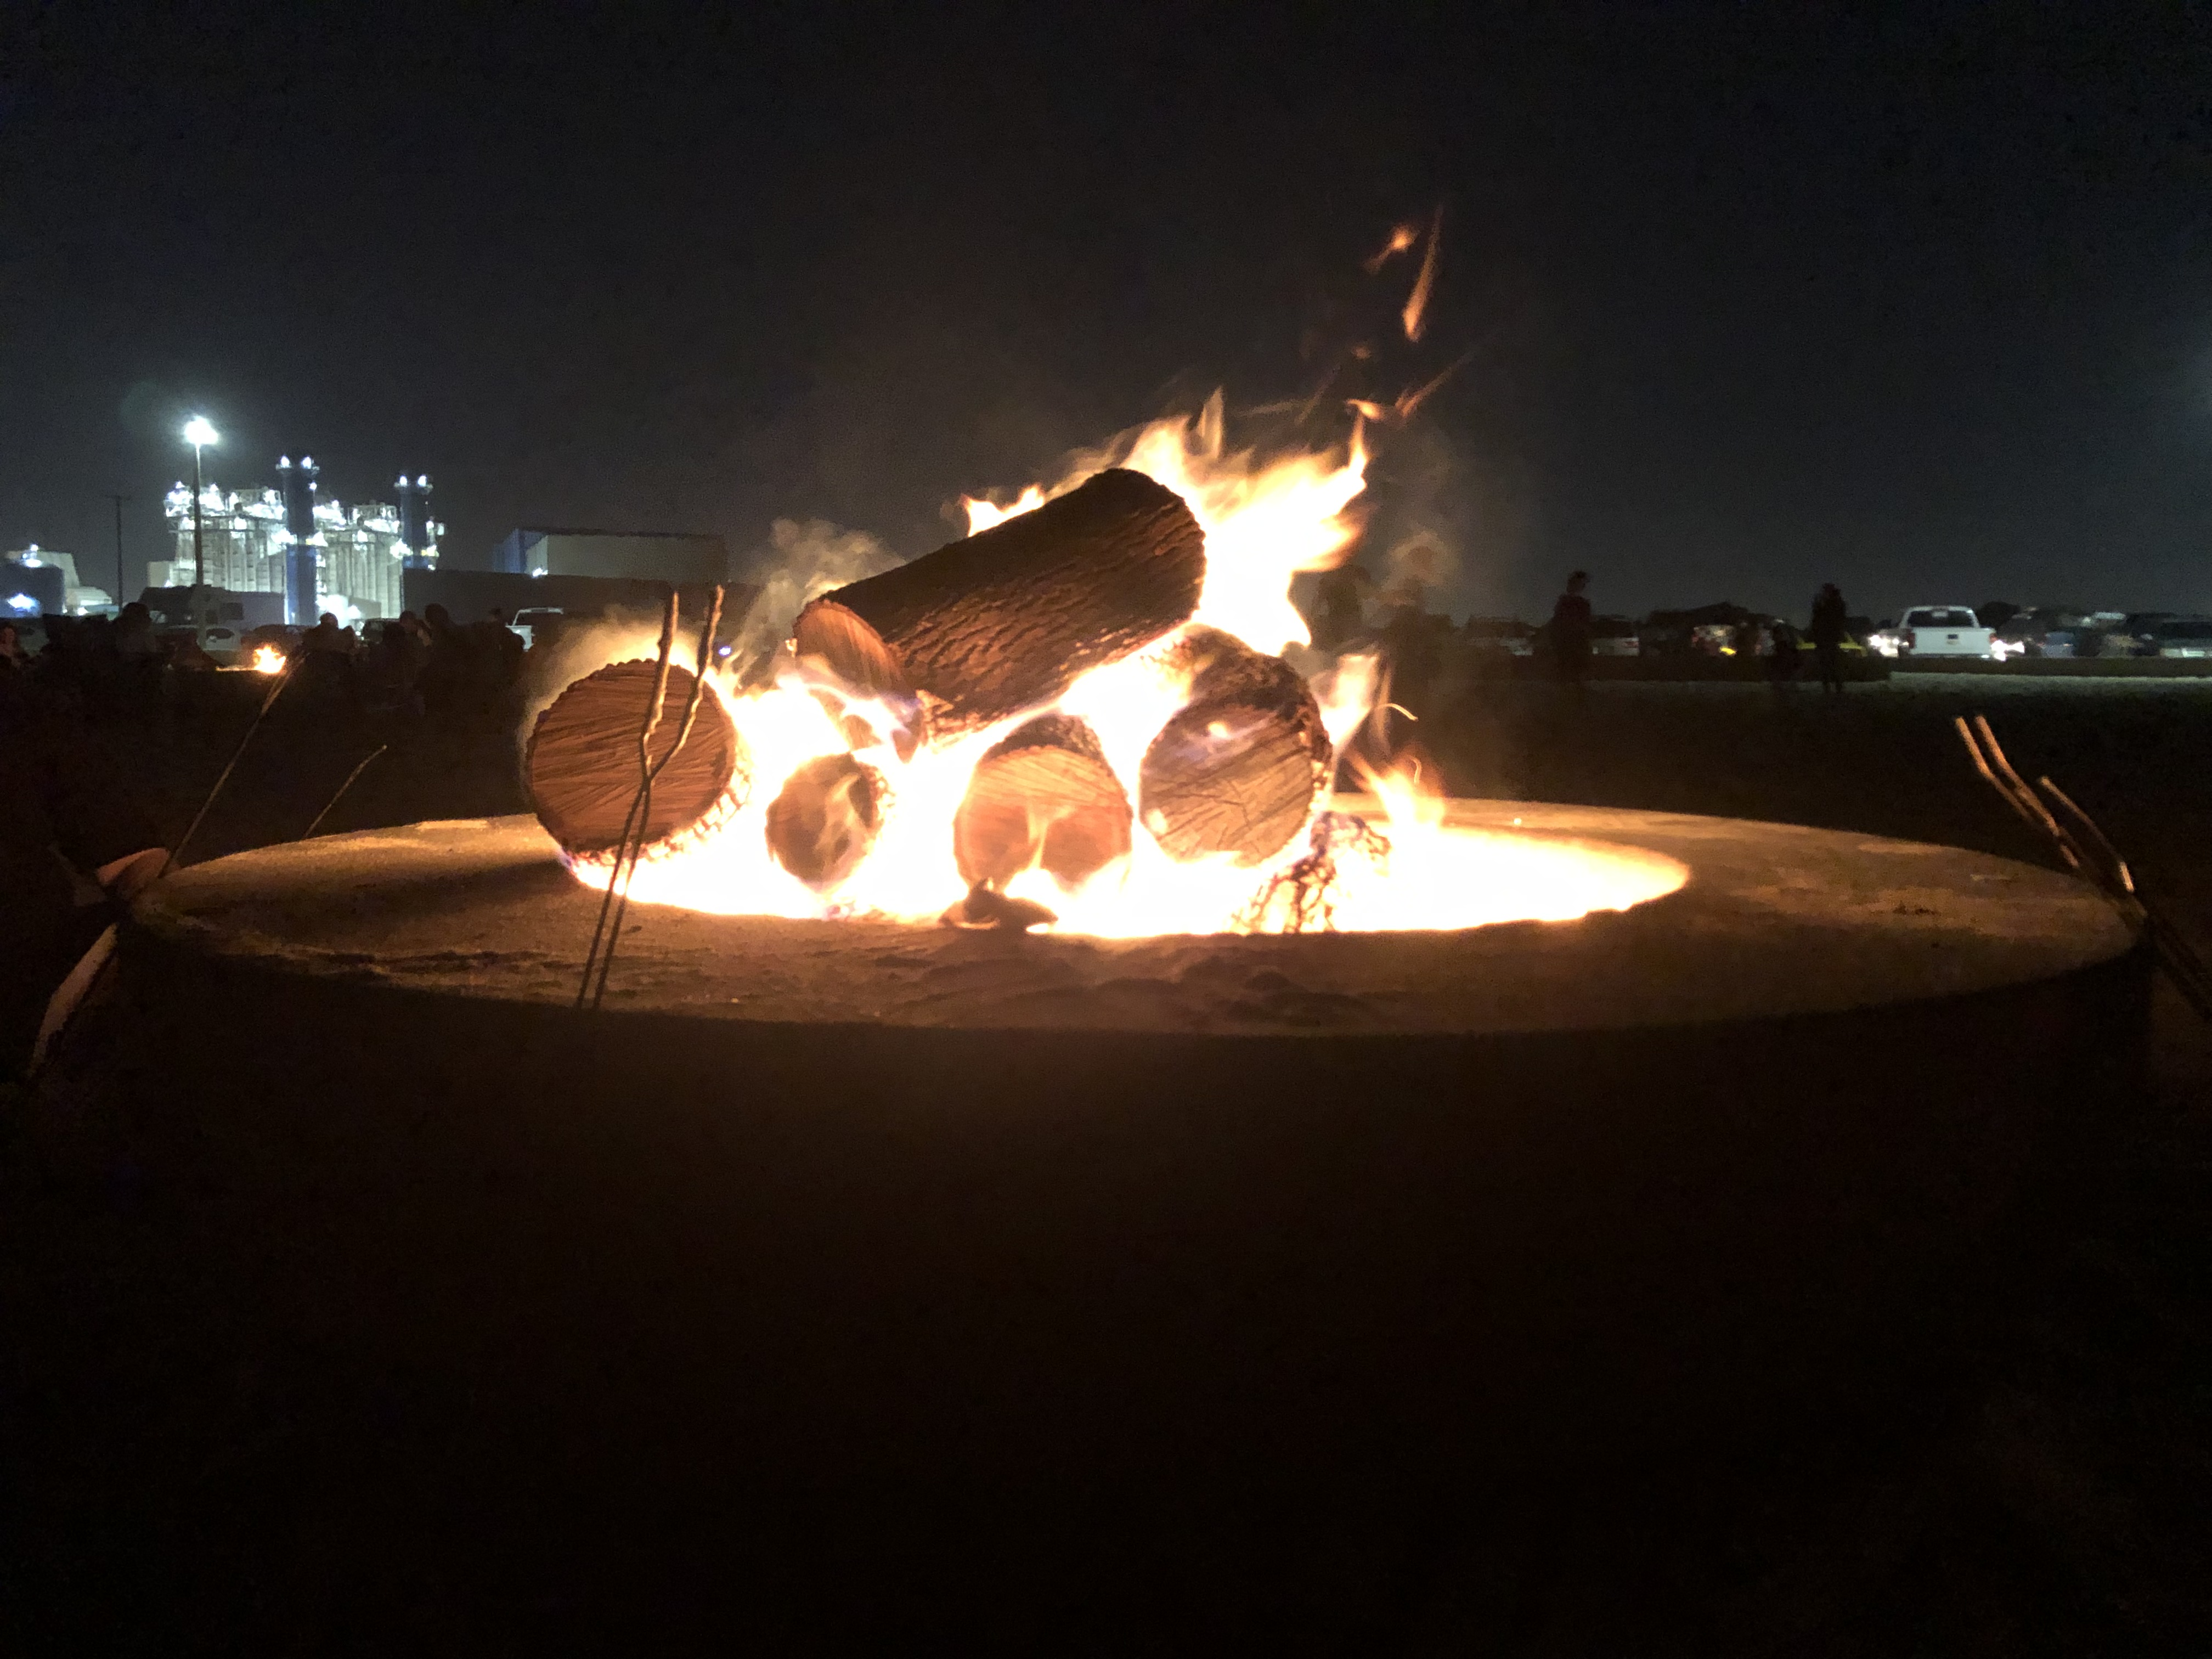
\includegraphics[scale=0.05]{bonfire}
\end{frame}

\begin{frame}{Practice: Classify the following as chemical or physical changes}
  \begin{enumerate}
  \item Melting solid gold into liquid gold
  \item Combining copper and tin to form bronze (an alloy)
  \item Electrolysis of water (H$_2$O) into hydrogen (H$_2$) gas and oxygen (O$_2$)
    gas
  \item Filtering algae from water
  \end{enumerate}
\end{frame}

\section{Potential and Kinetic Energy}

\begin{frame}{Whiteboard: Potential and Kinetic Energy}
\end{frame}

\section{Scientific Method}

\end{document}
